% !TeX spellcheck = en_GB
\chapter{\IfLanguageName{dutch}{Stand van zaken}{State of the art}}
\label{ch:stand-van-zaken}
% Tip: Begin elk hoofdstuk met een paragraaf inleiding die beschrijft hoe dit hoofdstuk past binnen het geheel van de bachelorproef. Geef in het bijzonder aan wat de link is met het vorige en volgende hoofdstuk.
In this chapter the state of affairs will be examined. As mentioned in the introduction, this part of the bachelor's thesis will be used to get an in-depth understanding of the four key themes that incorporate the changes in Windows Server 2019. First, for the key themes mentioned before, a basic understanding of what they are will be established together with how these have been implemented in the latest version of the \acrshort{os}.

\section{Hybrid cloud}
Hybrid Cloud is a topic that has gained more momentum over the past years. For organizations, this makes it a consistent topic of interest and makes it one of the keystone themes in Windows Server 2019. \autocite{MWST2018} It is with this in mind that it is discussed as an essential part of the bachelor's thesis. It is especially beneficial to know the advantages that this aspect offers to Windows Server since the latest version, how these improve workflow and how they can be leveraged by organizations, in particular, Delaware. To start with, the different types of clouds will be analysed and discussed in the following subsection.

\subsection{Types of cloud solutions}
The National Institute of Standards and Technology differentiates four types of clouds \autocite{Mell2011}:
\begin{itemize}
	\item Private Cloud
	\item Community Cloud
	\item Public Cloud
	\item Hybrid Cloud
\end{itemize}	
It is  however important to keep in mind that virtualization is not the same as cloud computing. While virtualization detaches computing environments from their physical infrastructure through software, cloud computing is a service that delivers computing resources on demand via a network. \autocite{Naeem2016}

\subsubsection{Private cloud}
A private cloud is an internal infrastructure in the cloud that is designated for usage by a single organization. It can however consist of multiple clients, albeit in the same organization. It is only accessible inside a private internal network or over the Internet for a selected amount of users than for the public. Private clouds can also be known by other names such as internal or corporate cloud. Their main advantage is the higher level of security and privacy . They offer this to organizations through the usage of in-house hosted infrastructure and additional company firewalls. The biggest disadvantage that comes with this added layer of security is the responsibility that is given to the \acrfull{it} team that manages the infrastructure that supports the private cloud. This means, on top of the additional in-house hosting cost, that they require the same amount of man-hours that come with the management of a traditional data centre. Keep in mind that in-house does not necessarily mean on-premise.
Still, the private cloud holds a great benefit compared to long-standing methods. As reported by IBM, an organization that saved more than \$1.5 billion by reducing their number of datacenters from 115 to 5. This was a direct result of the implementation of a private cloud. \autocite{Hofmann2010} 


\subsubsection{Community cloud}
When several organizations collaborate to meet the requirements that are demanded of the \acrshort{it} infrastructure, they are operating under a community cloud. This means that it can be managed in-house or by a third-party organization that operates inside the same community. This form of operation tackles one of the main problems of a private cloud. It shares the costs over multiple organizations, thus greatly reducing it for a single organization. Since they are operating inside the same community, they share the same concerns and will be subjected to the same requirements that can be imposed by a governing instance. 
This advantage over private clouds is only a partial improvement. This cost reduction as a result of sharing the infrastructure means a devaluation of security. Meaning that it is a viable alternative to  organizations that have some security concerns with the usage of a public cloud, but are willing to make some sacrifices in favour of lower costs. 
\newline
An example of this is described in an article \autocite{Yao2014} about how small hospitals in China, not all of which can provide their own infrastructure, could utilize a community cloud. These grass-roots healthcare institutions, that all operate within the same community, can share the cost and management of the cloud to provide an attractive hospital information solution to improve their service without the extensive cost nor the need for additional security concerns regarding confidential information in patient files.

\subsubsection{Public cloud}
Amazon Web Services, Oracle Cloud and Microsoft Azure are only some examples of public clouds. Most of these solutions are offered by corporations, like those mentioned above, who manage and operate their data centres and provide access to their cloud via the Internet. Thus eliminating the cost that is associated with the management and responsibility of a private cloud, where the \acrshort{it} department is responsible, and so significantly reduces the cost in equivalent use cases. Public clouds also provide the possibility for painless scalability and flexibility in comparison with private clouds, in which the hardware needs to be available in-house. This makes the public cloud ideal for temporary solutions.
\newline
\textcite{Singh2012} concluded, in a comparison between the cost and security of private and public clouds over three years, that although security can be a real concern in the usage of public cloud it should not be ruled out immediately without fully analysing the requirements of an organization, this with keeping in mind the major investment that comes paired with the usage and implementation of a private cloud.  
The different obstacles that securing a public cloud has are also addressed by \textcite{Ren2012}, in which there is a call for additional research about the subject to fully take advantage of the revelation that cloud computing is. 

\subsubsection{Hybrid cloud}
A hybrid cloud aims to be the solution for every business. It combines the higher level of security and privacy that is offered by the private cloud with easy scalability and flexibility that comes paired with the public cloud. In a hybrid cloud the organization manages a part of its cloud infrastructure in-house and a part out-house. As described in the book by \textcite{Sarna2010}, hybrid clouds enables large organizations to move their less sensitive information, like \acrfull{hr}, to the cloud. Thanks to the advantages of hybrid cloud their sensitive data, such as classified information about costumers or the organization, can remain in-house on private clouds or even on-premise for an additional layer of security. The connection between both the public and private cloud part of the hybrid cloud is generally accomplished through a \acrfull{vpn}.

\subsection{Hybrid cloud in Windows Server 2019}
%TODO Windows Admin Center

\section{Security}
With more than 53.000 reported incidents and 2.216 confirmed data breaches \autocite{Verizon2018}, security has become an essential part of \acrshort{it}. The importance of security directly translates into Windows Server 2019 through various parts of the \acrshort{os} that have either been reviewed to make them more resilient and accessible or new features which have been added to further improve security. In the following section all the major elements will be discussed, distributed among three subsections:
\begin{itemize}
	\item Windows Defender \acrfull{atp}
	\item Security with \acrfull{sdn}
	\item Shielded Virtual Machines
\end{itemize}

\subsection{Windows Defender \acrfull{atp}}
In a research study done by \textcite{Musto2017} \acrfull{wdatp} was scrutinized. When the endpoint security solution is implemented in Windows Server 2019, it requires additional licensing. Still, the efficiency with which it tackles security problems resulted in a 53\% \acrfull{roi}. The research reported that \acrshort{wdatp} reduced the risk of a breach by 40\%. It even enabled them to identify threats faster and resolve them in a more efficient fashion. In conclusion, the replacement of previous solutions with \acrlong{wdatp} reduced costs and made security teams more efficient. With the advent of Windows Server 2019, additional features have been added to \acrlong{wdatp} to ensure the safety of organizations in the years to come. The different components of \acrshort{wdatp} are described in the picture below. Those will not be individually reviewed here as this subject alone offers enough content for another bachelor's thesis.
\begin{figure}[hbt!]
	\centering
	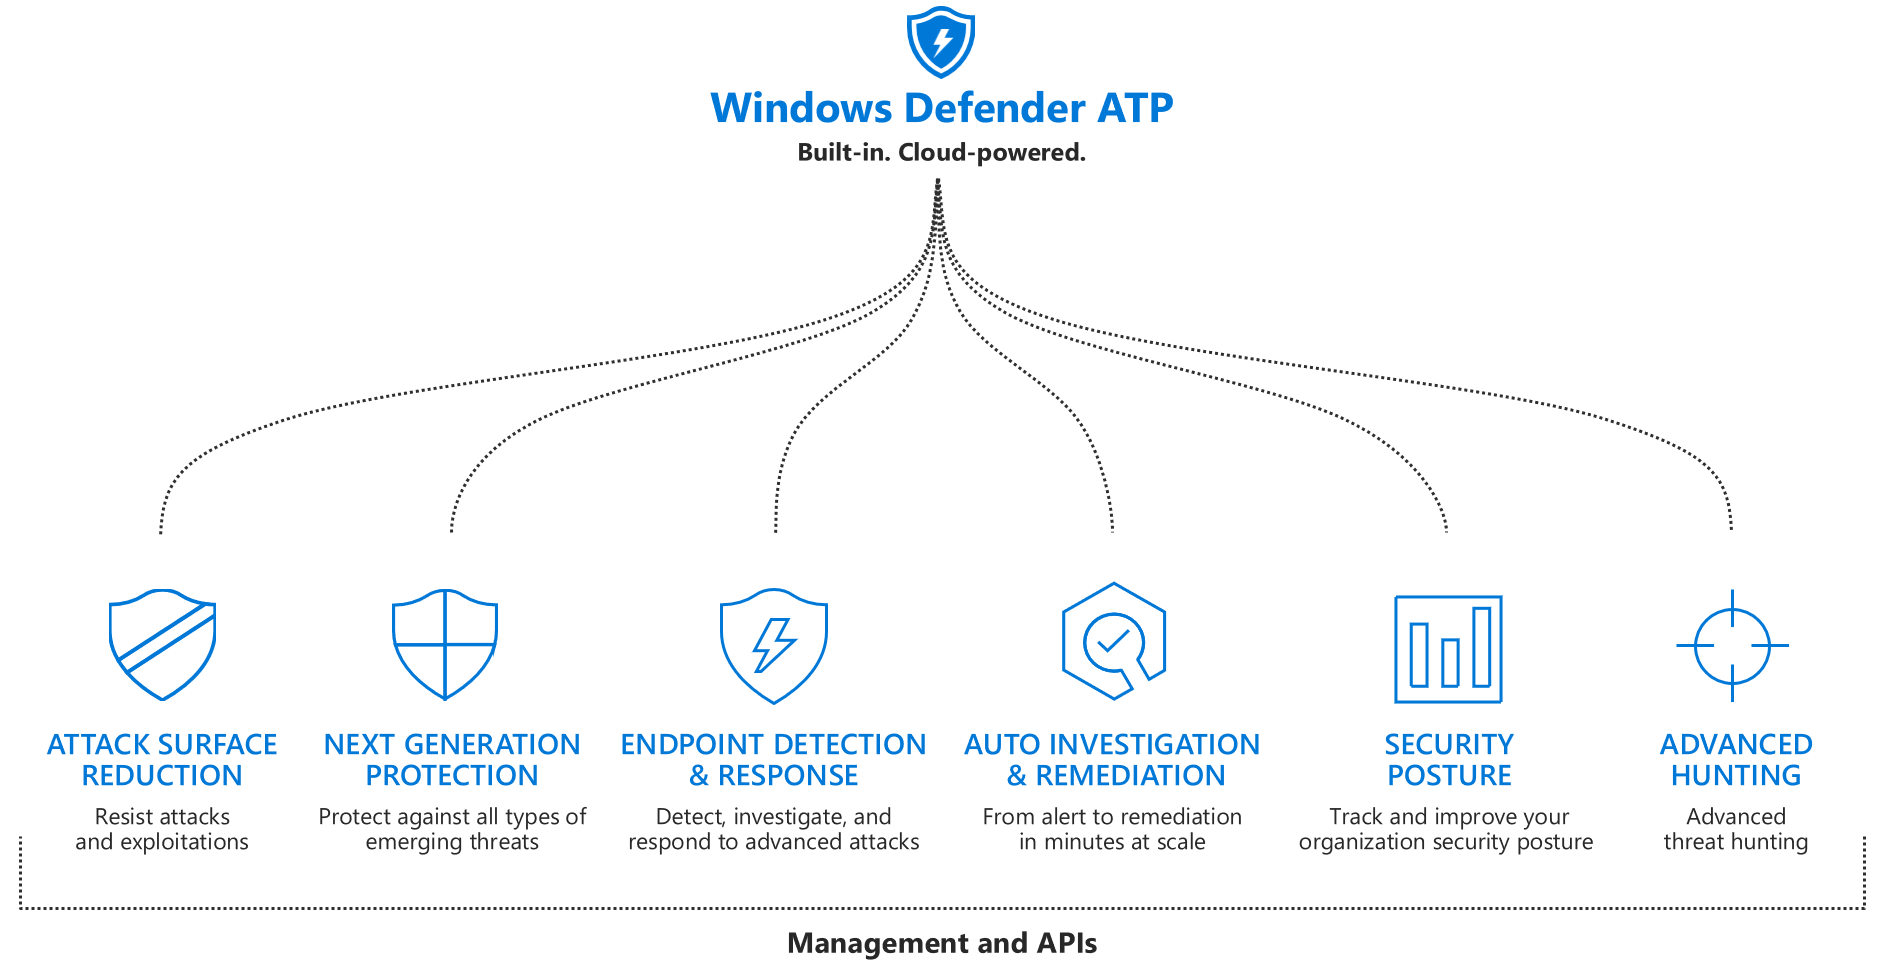
\includegraphics[width=\textwidth,height=6cm,keepaspectratio=true]{img/Windows-Defender-ATP.png}
	\caption[Components of \acrshort{wdatp}]{The different components of \acrlong{wdatp}. \autocite{Aslaner2018}}
	\label{fig:WDATPT2018}
\end{figure}

\subsection{Security with \acrfull{sdn}}
As described by \textcite{Shin2016}, \acrfull{sdn} is a state-of-the-art technology that enables developers to design advanced networks effortless. In Windows Server 2019 their have also been new development in this field, these can be boiled down to four features. The discussion of these will be constrained.
\begin{itemize}
	\item Encrypted networks
	\item Firewall auditing
	\item Virtual network peering
	\item Egress metering
\end{itemize} 

\subsubsection{Encrypted networks}
Encrypted networks, or more specifically virtual encrypted networks, enable the encryption of network traffic between different \acrlong{vm}s. It does this through the usage of \acrfull{dtls}. \acrshort{dtls} was built as close to \acrshort{tls} as possible \autocite{Modadugu2004}, which makes it ideal at securing connections. However, for the connection between \acrlong{vm}s \acrshort{dtls} is preferred, since these connections are delay sensitive. 

\subsubsection{Firewall auditing}
One of the new features in Windows Server 2019 is \acrshort{sdn} Firewall auditing. This means that the administrator is enabled to see if every part of his Firewall is as secure as is initially thought. When this feature is enabled every data stream that gets processed by the \acrshort{sdn} firewall, gets recorded. The logs can than be used in troubleshooting or archived for analysis. These can also be processed by using tools such as Power BI.

\subsubsection{Virtual network peering}
Virtual network peering allows you to combine two individual virtual networks. A coherent connection is made that represents itself as an individual one. This means the connection between both networks can be routed through the infrastructure backbone, this in term means that there is no need for a public gateway. Providing a more secure connection, while no additional downtime is accumulated when peering the networks.

\subsubsection{Egress metering}
Egress metering for \acrshort{sdn} enables an administrator to monitor the consumption on outgoing connections. Windows Server 2019 also makes a distinction between traffic that leaves the virtual network and the data centre, in comparison to traffic that stays within the data centre. 

\subsection{Shielded Virtual Machines}
One of the requirements to run a Shielded \acrfull{vm} is a \acrfull{hgs}. Since Windows Server 2019 it is possible to run Shielded \acrshort{vm}s on machines with irregular connection to the \acrshort{hgs}. This can be done by leveraging the two new features. 

\begin{description}
	\item[Fallback \acrshort{hgs}] Provide a redundant connection in case the primary \acrshort{hgs} can not be reached.
	\item[Offline Mode] Once a shielded \acrshort{vm} has been setup it can be started up seeing the security configuration remains unchanged.
\end{description}

Another new feature is the addition of support for Ubuntu, Red Hat Enterprise Linux and SUSE Linux Enterprise Servers inside Shielded \acrshort{vm}s. 

\section{Application platform}
% TODO Application Platform
%\subsection{Linux containers on Windows}
%\subsection{Building Support for Kubernetes}
%\subsection{Container improvements}
%\subsection{Encrypted Networks}
%\subsection{Network performance improvements for virtual workloads}
%\subsection{Low Extra Delay Background Transport}
%\subsection{Windows Time Service}
%\subsection{High performance SDN gateways}
%\subsection{New Deployment UI and Windows Admin Center extension for SDN}
%\subsection{Persistent Memory support for Hyper-V VMs}

\section{Hyper-converged infrastructure}
% TODO HCI
\section{Conclusion}
% TODO Conclusion